%!TEX root = ../main.tex
\subsection{Utilizing the XCanPs}
\label{sub:TestingCANStack_BareMetal}
\mikkel{Changed!}
A CAN controller needs to be used when connecting a Zybo to a CAN bus.
XCanPs is a CAN controller built-in to the Zybo.
This section will seek to develop a PL architecture for the Zybo that allows for utilization of the XCanPs.
Furthermore it will describe the implementation of software that has the following functionality.
\begin{itemize}
\item Receiving and sending of frames.
\item Creating the message ID.
\item Decoding of the message ID.
\item Handling interrupts from buttons and a GPIO port.
\item Controlling the LEDs.
\item Accepting and ignoring messages according to a subscription list.
\end{itemize}
Some of the functionalities are not needed in the finished version of the system, but will be implemented for testing and debugging purposes.
% This section includes the design and development of hardware and software in order to realize the CAN network.
% This software and hardware co-design was developed firstly to establish a basic CAN network between a number of Zybos and secondly to prove and test the functionality of the CAN stack designed for this project.
% It was also meant to be the basis for the development of the CAN controller part of the full system but in the end it was only used for testing purposes, as described in section \ref{sub:CAN_Bus_Tests}.

\subsubsection*{Architecture}
To use the XCanPs these need to be enabled in the Zynq PS.
Interrupts were also enabled along with adding an AXI GPIO port connected to a PMOD connector to allow for externally triggered interrupts to the system.
Additional AXI GPIO cores for LEDs and buttons were added for debugging and testing purposes.
The architecture can be seen it figure \ref{fig:CAN_Testing_Architecture}. 
It is simple, but adequate to meet the purpose of basic communication between nodes.

\begin{figure}[h!]
	\centering
	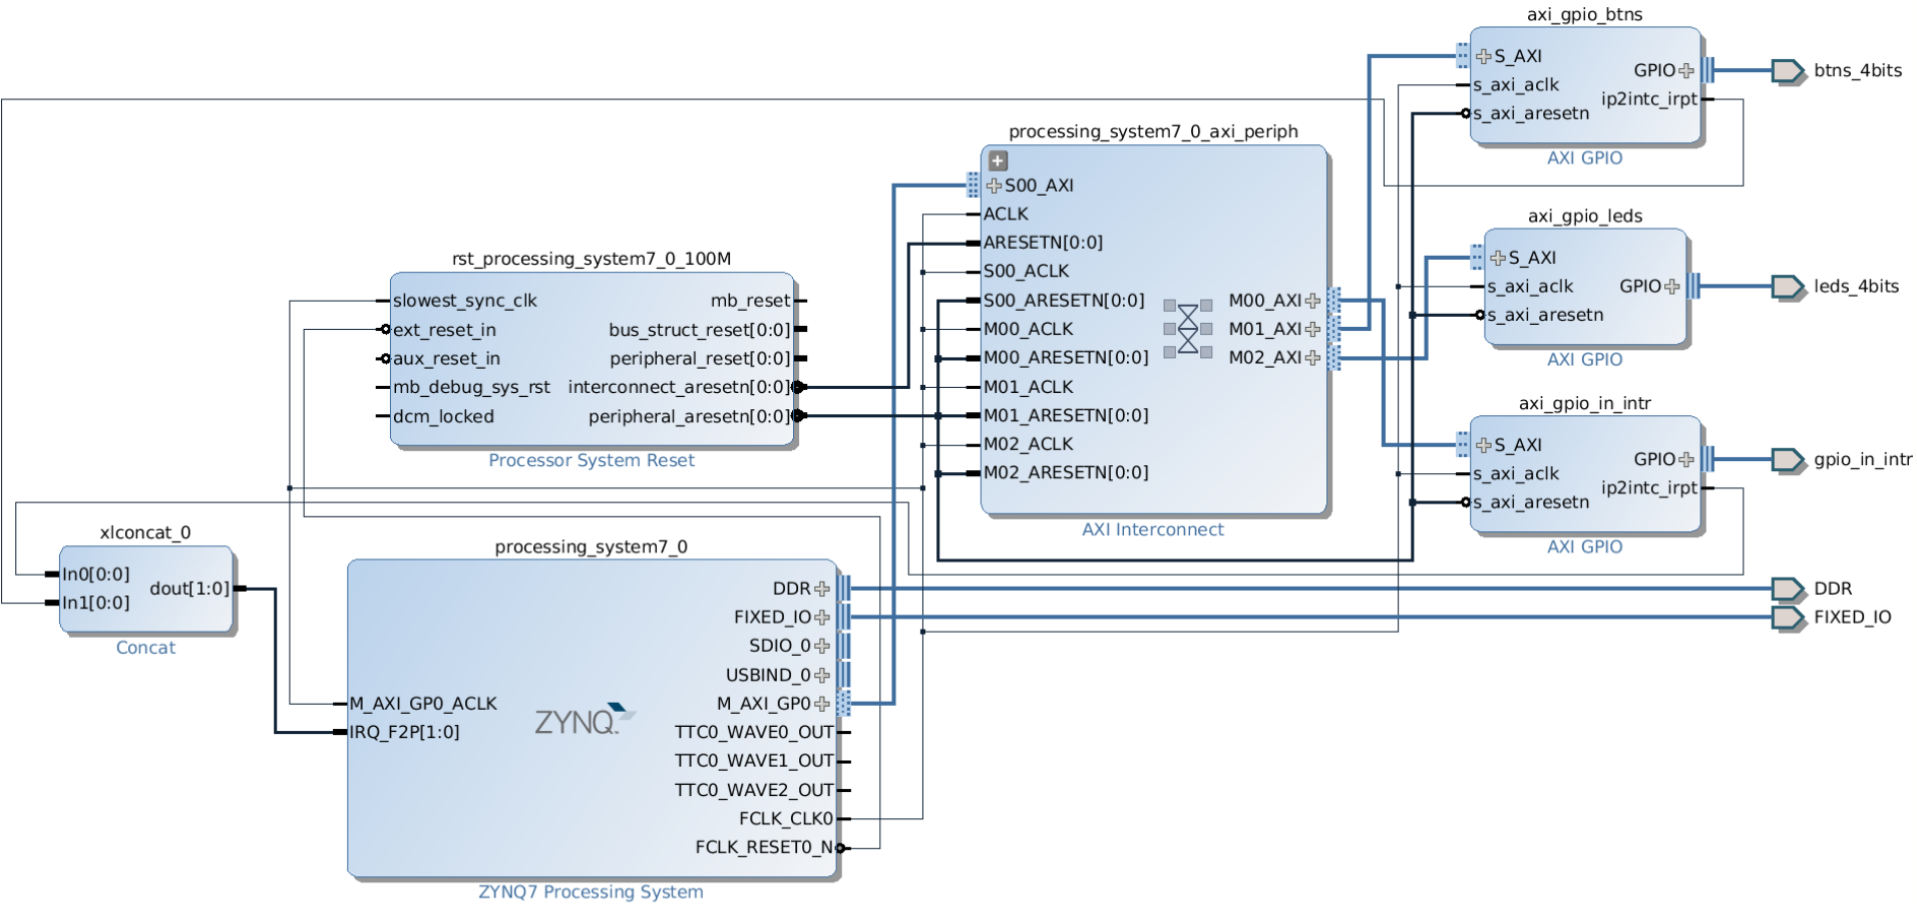
\includegraphics[width = 1\linewidth]{graphics/Zybo_BasicTestingArchitecture_for_CAN.png}
	\caption{Block diagram of the architecture in Vivado.}
	\label{fig:CAN_Testing_Architecture}
\end{figure}

\subsubsection*{Software}\label{sub:Basic_SourceCode}
Xilinx provides example code for the XCanPs in \texttt{xcanps\_polled\_example.c} \cite{xcanps}.
This is used as a basis for the developed software.
The code was rewritten to give the wanted functionality.

\subsubsection*{Sending Frames}
Figure \ref{fig:SeqDiagram_SendFrame} shows the procedure of sending a frame to the CAN network containing data, which makes use of the protocol function \texttt{createMsgID()}.
Its purpose is to create a message ID by putting together the new message bit, the node ID and the message type.
In the final implementation of the system the message ID would be provided by the software running in the userspace.
Afterwards the massage ID and dummy data are put into a \texttt{TxFrame}.
The \texttt{TxFrame} will be sent when the FIFO has space.
The actual sending is done with a call to the XCanPs function \texttt{XCanPs\_Send()}.

\subsubsection*{Receiving Frames}
The procedure of receiving a frame is shown in figure \ref{fig:SeqDiagram_RecvFrame}.
The node calls the \texttt{RecvFrame()} function and waits in a loop until it receives a frame.
Then it checks the subscriptions in order to determine if the message is addressed to the node using the function \texttt{amISubscribed()}.
This function makes use of an array containing the messages IDs that the node should accept when a message is being transmitted through the network.
\begin{figure}[h!]
	\centering
	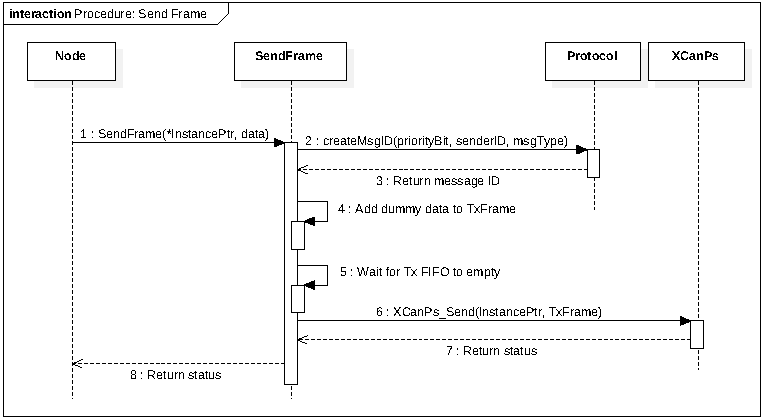
\includegraphics[width = 1\linewidth]{graphics/SeqDiagram_SendFrame.pdf}
	\caption{The sequence diagram of the process of sending a frame.}
	\label{fig:SeqDiagram_SendFrame}
\end{figure}

\begin{figure}[h!]
	\centering
	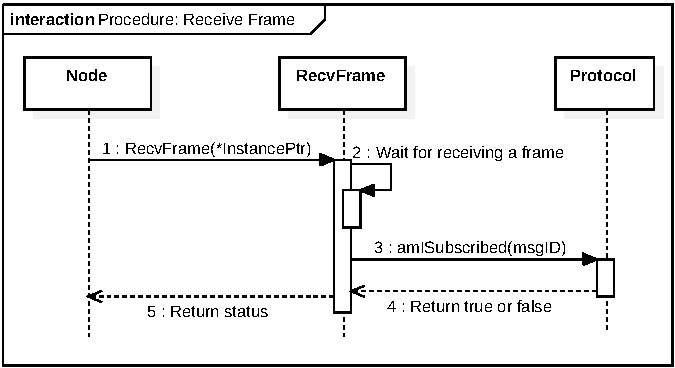
\includegraphics[width = 1\linewidth]{graphics/SeqDiagram_RecvFrame.pdf}
	\caption{The sequence diagram of the process of receiving a frame.}
	\label{fig:SeqDiagram_RecvFrame}
\end{figure}
